%%%%%%%%%%%%%%%%%%%%%%%%%%%%%%%%%%%%%%%%%%%%%%%%%%%%%%%%%%%%%%%%%%%%%%%%%%%%%%%%%%%%%%%%%%%%%%

%%%%%%%%%%%%%%%%%%%%%%%%%%%%%%%%%%%%%%%%%%%%%%%%%%%%%%%%%%%%%%%%%%%%%%%%%%%%%%%%%%%%%%%%%%%%%% 

%\documentclass{beamer} %voce pode usar este modelo tambem
\documentclass[handout,t]{beamer}
\usepackage{graphicx,url}
\usepackage[brazil]{babel}   
\usepackage[utf8]{inputenc}
\batchmode
% \usepackage{pgfpages}
% \pgfpagesuselayout{4 on 1}[letterpaper,landscape,border shrink=5mm]
\usepackage{amsmath,amssymb,enumerate,epsfig,bbm,calc,color,ifthen,capt-of}
\usetheme{Berlin}
\usecolortheme{whale}

%-------------------------Title information------------------------------------------------
\title[Where and why are temperature forecasts faulty?]{Where and why are temperature forecasts faulty?}
\subtitle{Data Expo 2018}
\date{July 30, 2018}
\author[Matt Higham, Erin Howard]{Matt Higham \\ Erin Howard}

%-------------------------Logo na parte de baixo do slide------------------------------------------
\pgfdeclareimage[height=1.5cm]{senac-logo}{logo.pdf}
\logo{\pgfuseimage{senac-logo}\hspace*{0.5cm}\vspace*{-0.5cm}}

%-------------------------Este código faz o menuzinho bacana na parte superior do slide------------
%\AtBeginSection[]
%{
%  \begin{frame}<beamer>
%    \frametitle{Outline}
%    \tableofcontents[currentsection]
%  \end{frame}
%}
\beamerdefaultoverlayspecification{<+->}
% -----------------------------------------------------------------------------
\begin{document}
% -----------------------------------------------------------------------------

%---Gerador de Sumário---------------------------------------------------------
\frame{\titlepage}
\section{MAP TITLE}
\begin{frame}{MAP TITLE}
  \begin{center}
  \vspace{-0.25in}
  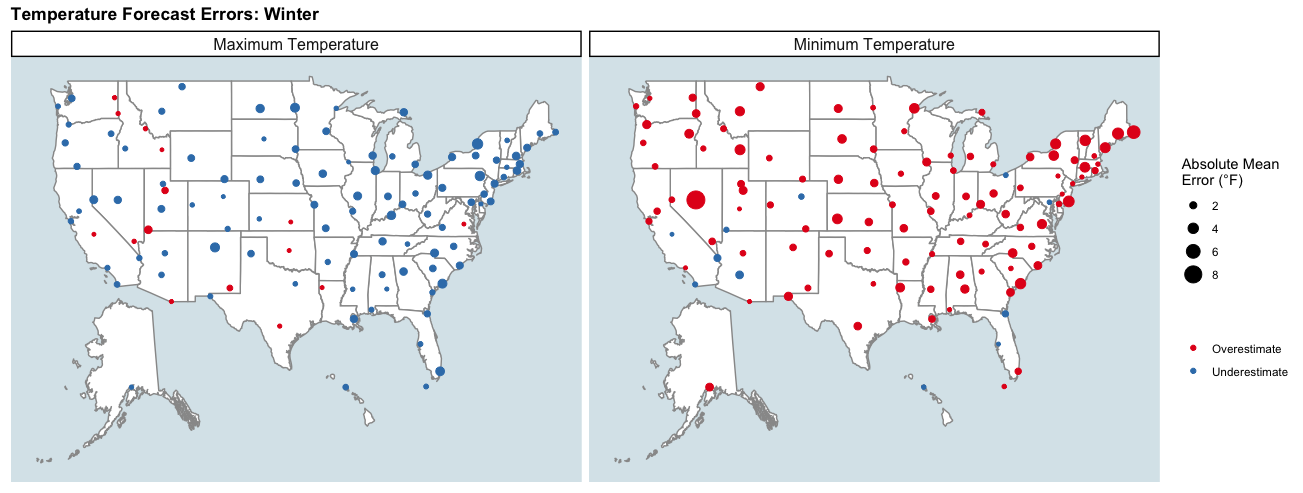
\includegraphics[scale=0.25]{Both_winter_maps.png}
  \end{center}
\end{frame}
%---Fim do Sumário------------------------------------------------------------


% -----------------------------------------------------------------------------
\section{DISTANCE TITLE}
\begin{frame}{DISTANCE TITLE}
  \begin{center}
  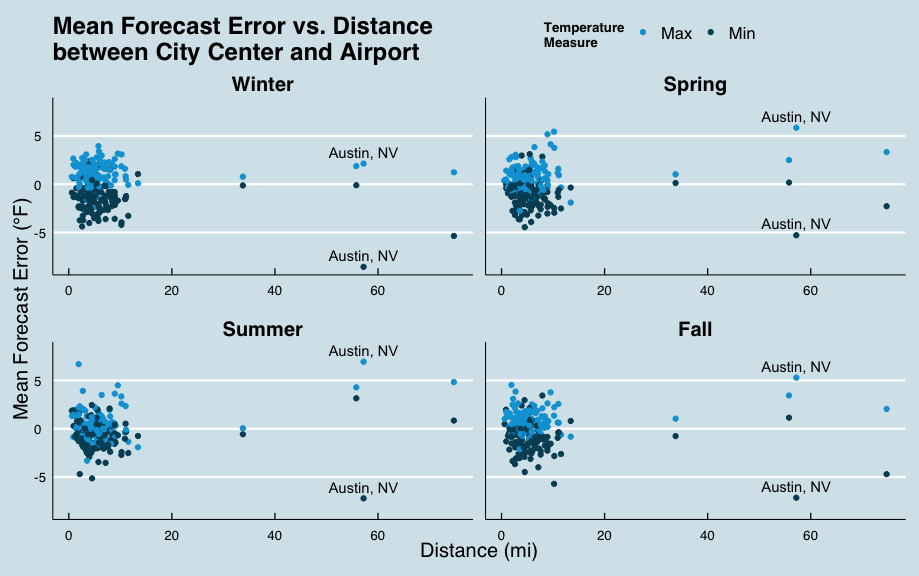
\includegraphics[scale=0.25]{Distance_Plot_Poster.png}
  \end{center}
\end{frame}
%------------------------------------------------------------------------------

%------------------------------------------------------------------------------
\section{BIAS VARIANCE TITLE}
\begin{frame}{BIAS VARIANCE TITLE}
  \begin{center}
  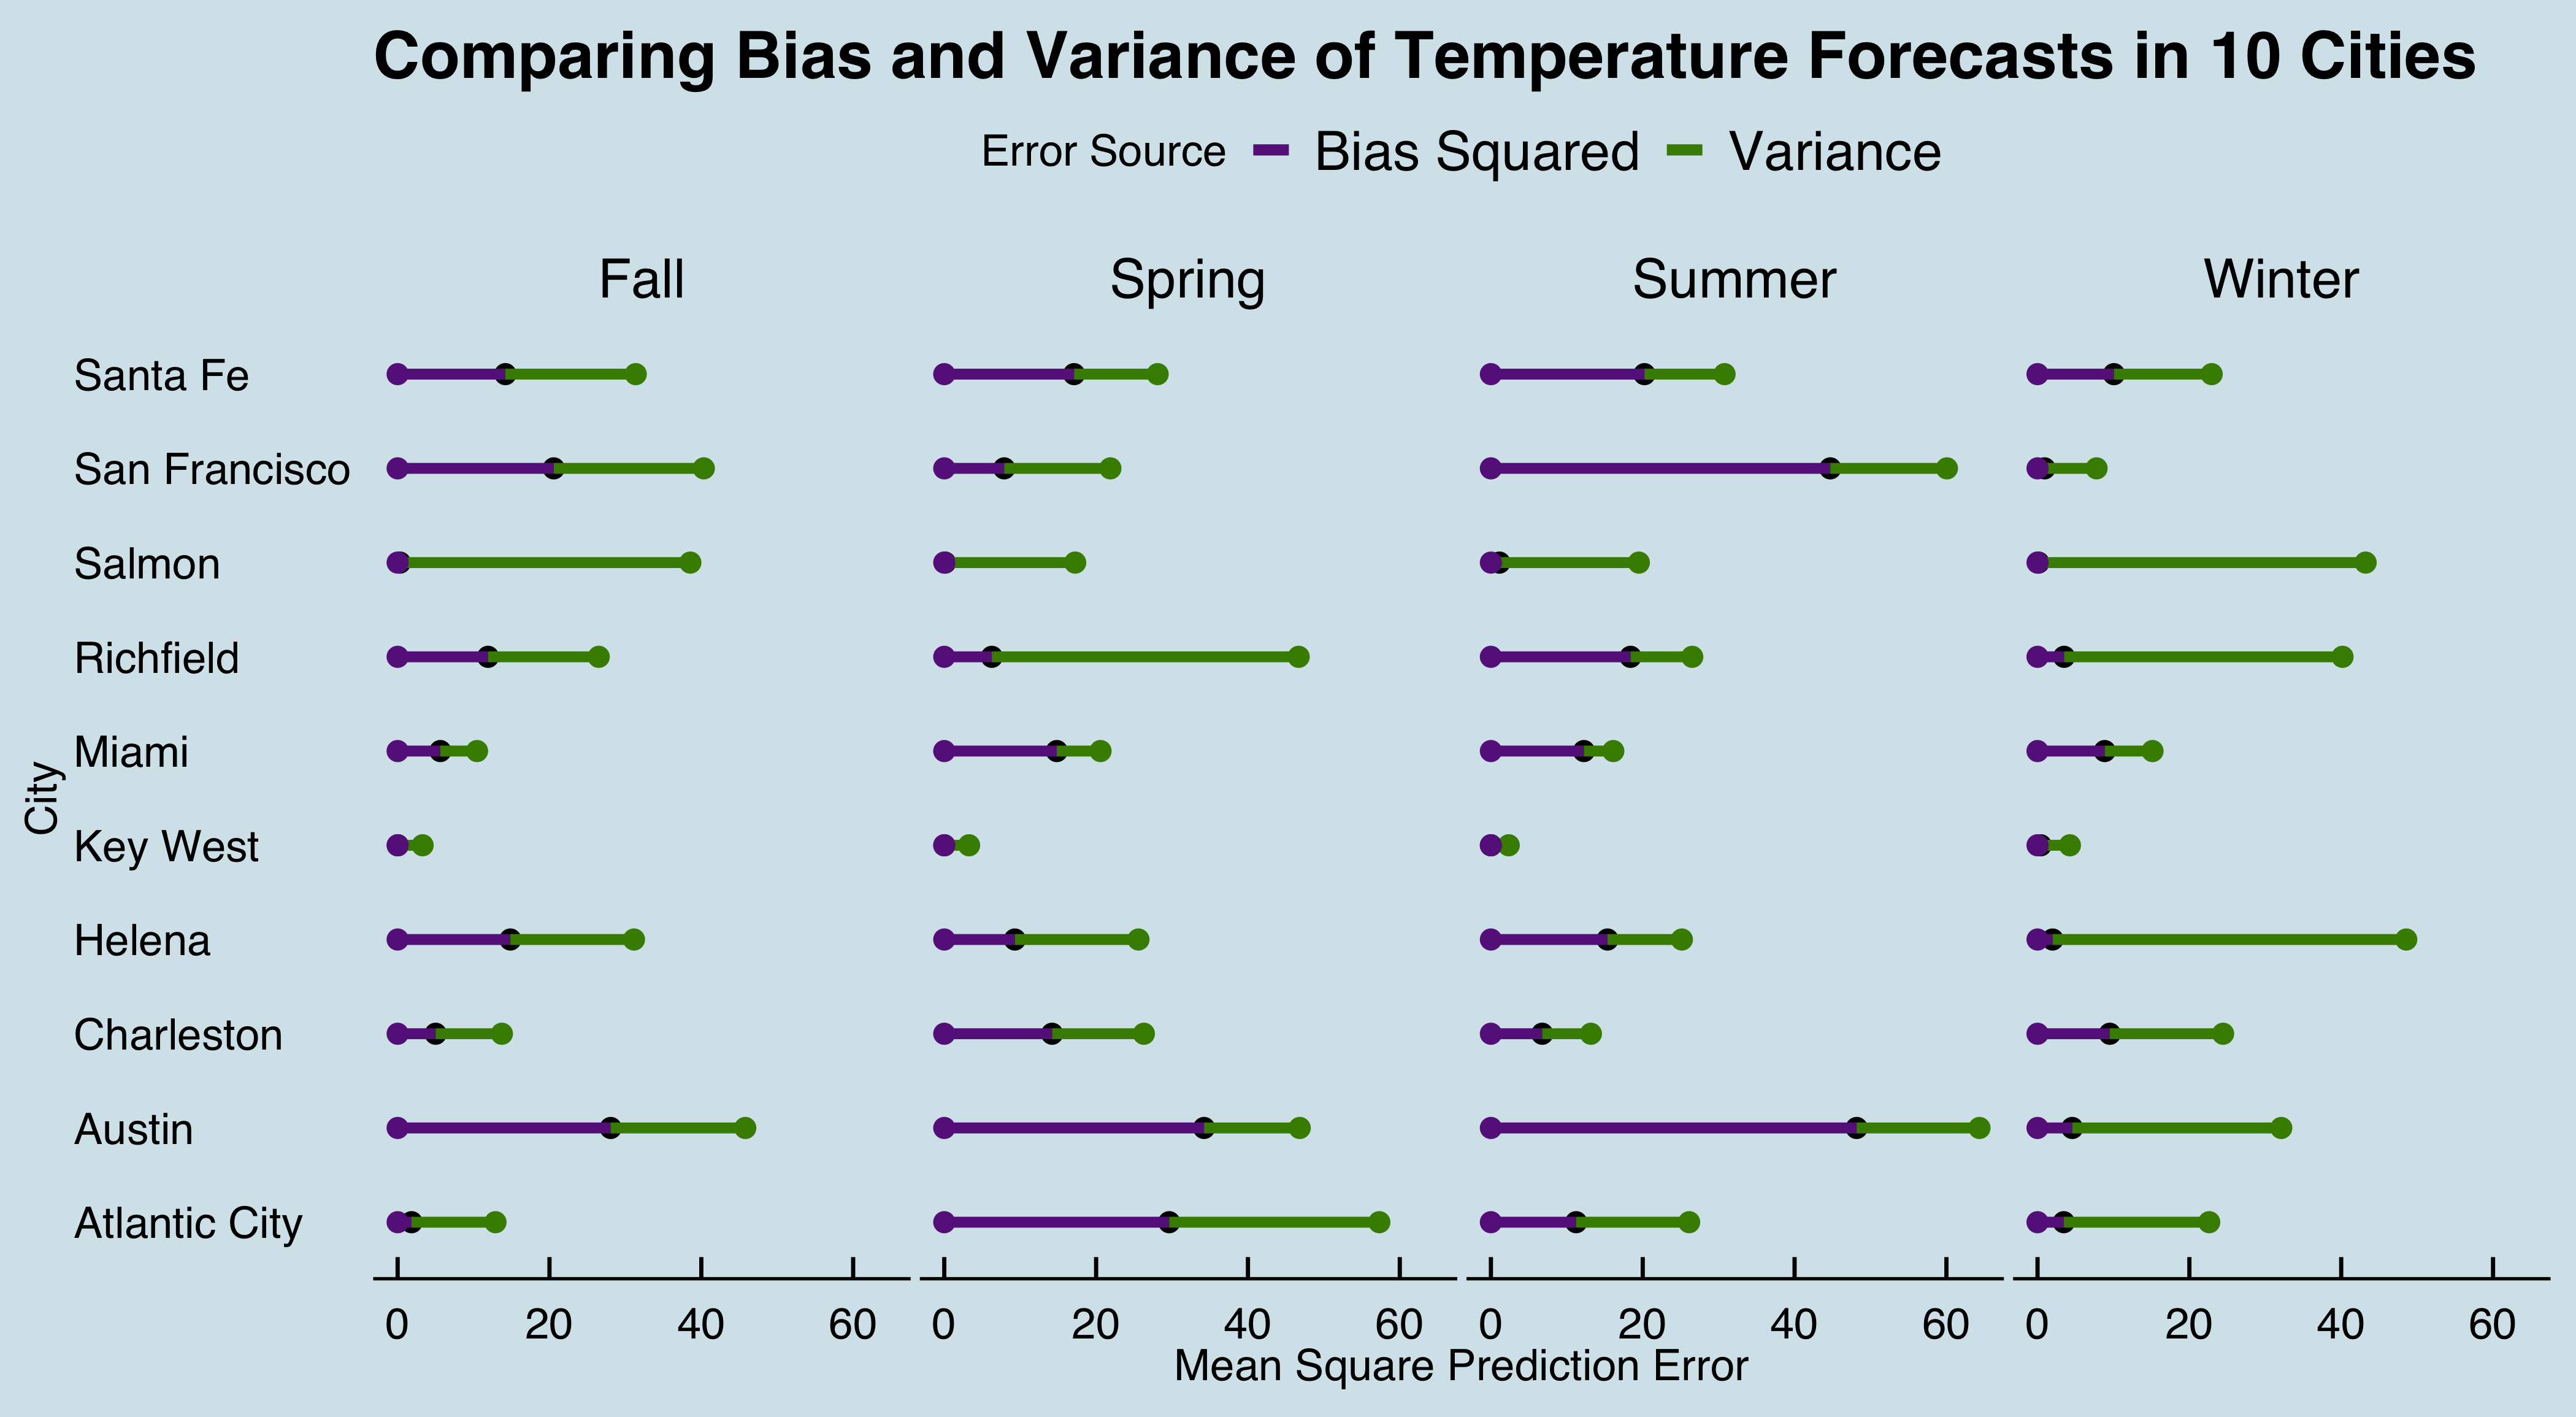
\includegraphics[scale=0.06]{BiasVarGraph.png}
  \end{center}
\end{frame}
%------------------------------------------------------------------------------

%------------------------------------------------------------------------------
\section{Metodologia}
\begin{frame}{Metodologia}
Metodologia minuciosamente aqui.
\end{frame}
%------------------------------------------------------------------------------

%------------------------------------------------------------------------------
\section{Considerações e Resultados}
\begin{frame}{Considerações e Resultados}
%consideraçoes e resultados
Resultados e considerações do trabalho  
\end{frame}
%------------------------------------------------------------------------------

%------------------------------------------------------------------------------
\section{Referencias}
\begin{frame}{Referencias}
  Suas referencias bibliográficas aqui, siga o modelo ABNT.
\end{frame}
%------------------------------------------------------------------------------

%------------------------------------------------------------------------------
\section{Agradecimentos}
\begin{frame}{Agradecimentos}
Agradeço a todos que colaboraram  para realizaç~ao deste projeto.
Agradeço ao Alexandre Bencz pelo assembly de cada dia.
Agradeço ao Sonata Arctica, Avantasia, Mago de Oz, Cain's Offering, e todas as outras bandas de Power Metal. 	
\end{frame}
%------------------------------------------------------------------------------

%------------------------------------------------------------------------------
\subsection{Sites legais}
\begin{frame}{Sites legais}
  Want to know more? See!
  \begin{itemize}
    \item Browse in my page \url{http://www.ezefranca.com}.
    \item Browse on BCC page \url{http://www.sp.senac.br/bcc}.
    \item Thanks WriteLaTeX from Support! \url{http://www.writelatex.com}.
  \end{itemize}
  
\end{frame}
%------------------------------------------------------------------------------

% -----------------------------------------------------------------------------
\end{document}
%-----------------------------------------------Este comentario nunca aparecera